\documentclass[russian]{article}
\usepackage[T2A,T1]{fontenc}
\usepackage[utf8]{inputenc}
\usepackage[landscape]{geometry}
\geometry{verbose,tmargin=2cm,bmargin=2cm,lmargin=2cm,rmargin=2cm}
\usepackage[russian]{babel}
%\usepackage{pdflscape}
\usepackage{amsfonts}
\usepackage{amsmath}

\usepackage[pdftex]{graphicx}

\begin{document}

\section{}
$p_1 .. p_n \in \mathbb{Q},$ $m$ -- общий знаменатель этих чисел. Тогда:
$$\int R\left(x, \left(\frac{ax + b}{cx + d}\right)^{p_1}, .. \left(\frac{ax + b}{cx + d}\right)^{p_n}\right) dx = \left[t^m = \frac{ax + b}{cx + d} \right] = \int R(t) dt$$

\section{}
Пунктирные линии обозначают разбор случаев. Сплошные -- разложение в линейную комбинацию.

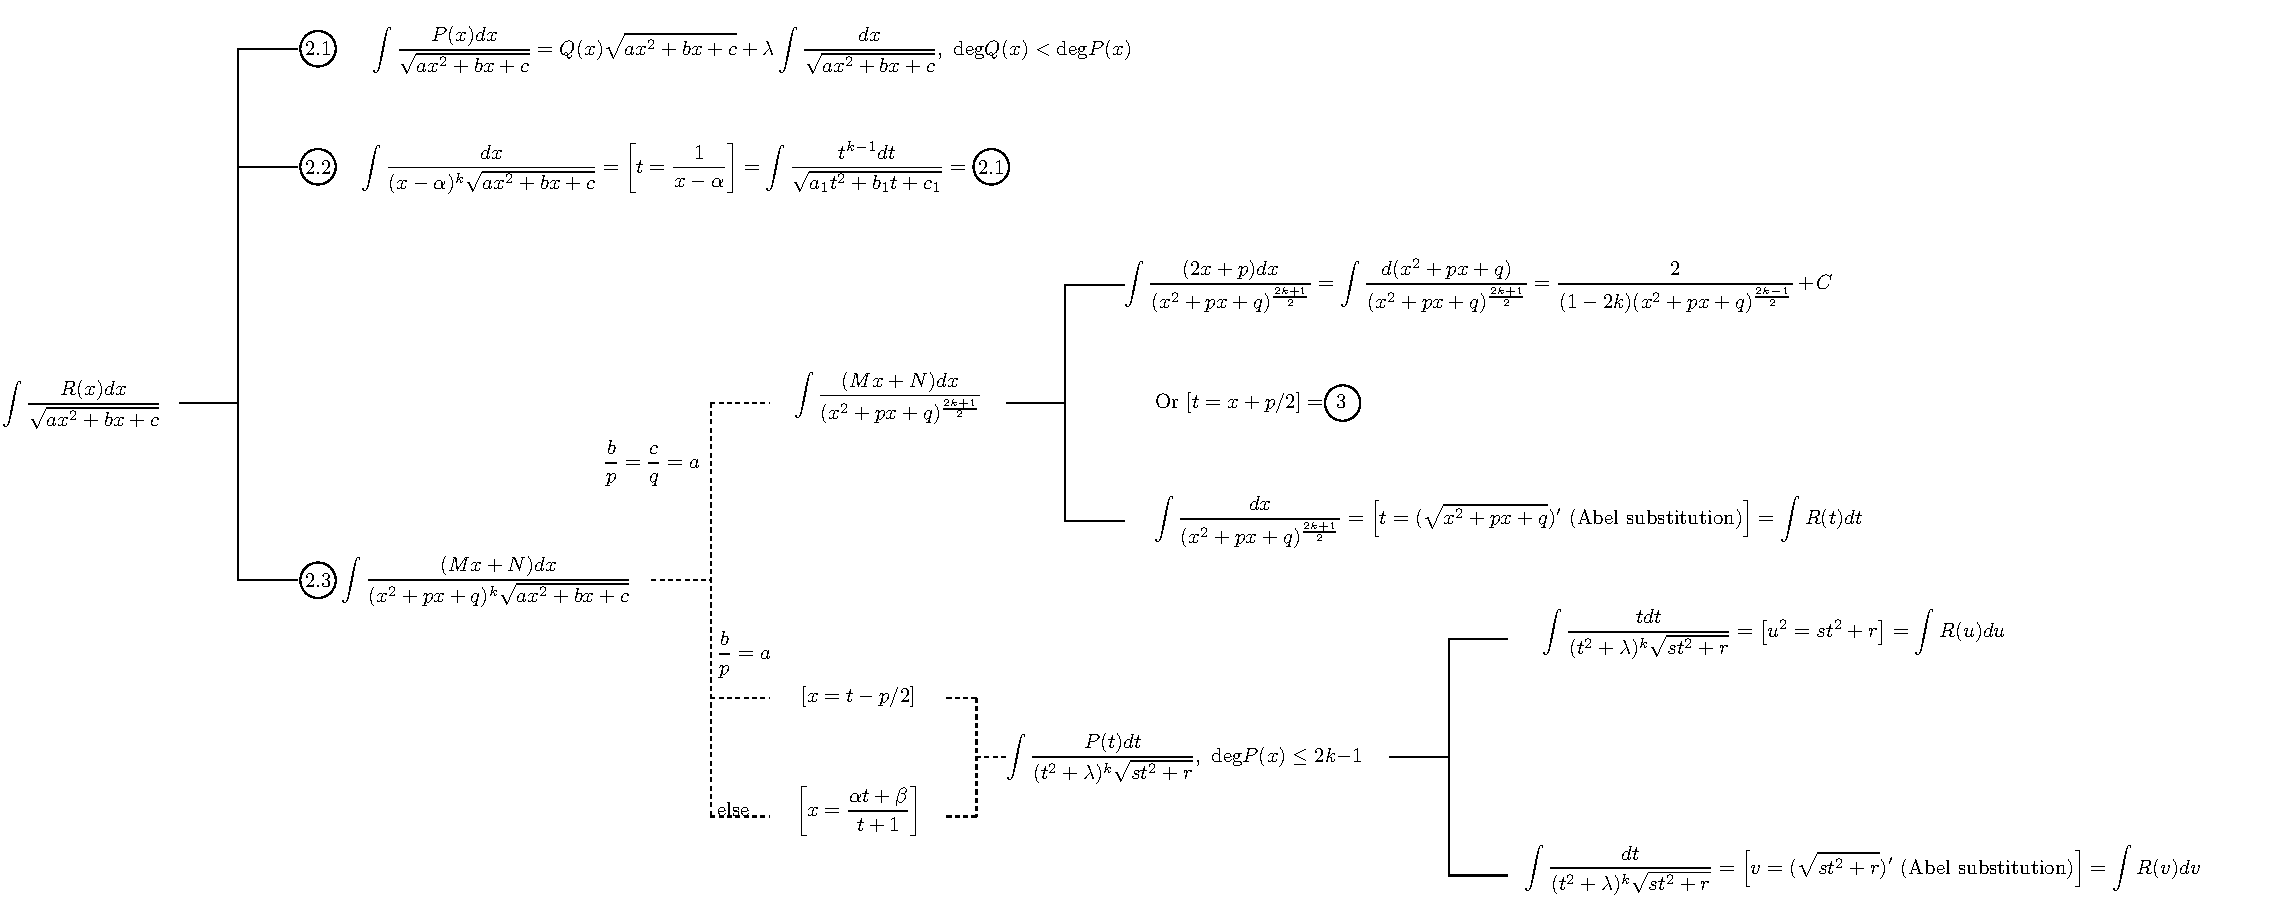
\includegraphics[width=\textwidth]{pic/irrational_scheme.pdf}


\textit{Иногда} удобно использовать тригонометрические замены, предварительно выделив полный квадрат под корнем:
\begin{itemize}
 \item $$ \int R(x, \sqrt{p^2 - x^2}) dx = \left[ x = p \sin t \text{ или } x = p \cos t  \text{ или } x = p \th p\right]$$
 \item $$ \int R(x, \sqrt{x^2 - p^2}) dx = \left[ x = \frac{p}{\cos t} \text{ или } x = p \ch t  \right]$$
 \item $$ \int R(x, \sqrt{x^2 + p^2}) dx = \left[ x = p \tg t \text{ или } x = p \sh t  \right]$$
\end{itemize}

\section{}
$$\int x^m (ax^n + b)^p dx, \text{ где } m, n, p \in \mathbb{Q}$$
\begin{itemize}
 \item Если $p \in \mathbb{Z}$, то $x = t^N$, где $N$ -- общий знаменатель $m$ и $n$.
 \item Если $\frac{m + 1}{n} \in \mathbb{Z}$, то $t^s = ax^n + b$, где $s$ -- знаменатель $p$.
 \item Если $\frac{m + 1}{n} + p \in \mathbb{Z}$, то $t^s = a + bx^{-n}$, где $s$ -- знаменатель $p$.
 \item В остальных случай интеграл не выразить через элементарные функции.
\end{itemize}

\end{document}
